\documentclass[10pt,twocolumn,letterpaper]{article}

\usepackage{cvpr}
\usepackage{times}
\usepackage{epsfig}
\usepackage{graphicx}
\usepackage{amsmath}
\usepackage{amssymb}
\usepackage{enumitem}
\usepackage[table,xcdraw]{xcolor}

\usepackage[
backend=bibtex,
sorting=none
]{biblatex}
\addbibresource{references.bib}

% Include other packages here, before hyperref.

% If you comment hyperref and then uncomment it, you should delete
% egpaper.aux before re-running latex.  (Or just hit 'q' on the first latex
% run, let it finish, and you should be clear).
\usepackage[breaklinks=true,bookmarks=false]{hyperref}

\cvprfinalcopy % *** Uncomment this line for the final submission

\def\cvprPaperID{****} % *** Enter the CVPR Paper ID here
\def\httilde{\mbox{\tt\raisebox{-.5ex}{\symbol{126}}}}

% Pages are numbered in submission mode, and unnumbered in camera-ready
%\ifcvprfinal\pagestyle{empty}\fi
\setcounter{page}{1}

\newcommand{\comment}[1]{}

\begin{document}

%%%%%%%%% TITLE
\title{Unsupervised Speaker Identification}

\author{Thivakkar Mahendran\\
University of Massachusetts Amherst\\
%Institution1 address\\
{\tt\small tmahendran@umass.edu}
% For a paper whose authors are all at the same institution,
% omit the following lines up until the closing ``}''.
% Additional authors and addresses can be added with ``\and'',
% just like the second author.
% To save space, use either the email address or home page, not both
\and
Varun Prasad\\
University of Massachusetts Amherst\\
%First line of institution2 address\\
{\tt\small varunanantha@umass.edu}
}

\maketitle
%\thispagestyle{empty}

%%%%%%%%% ABSTRACT
\begin{abstract}
   There have been massive improvements in speech recognition software in recent years, as evidenced by the rise in popularity of digital/voice assistants. Despite these advances, these technologies are sub-par when it comes to detecting and distinguishing between multiple speakers in noisy conditions. The objective of this project is to build a deep learning system for automatic speaker identification that can effectively distinguish which person is speaking at a specific time in a conversational setting of multiple people. We make use of a combination of supervised and unsupervised learning techniques to achieve this.
\end{abstract}

%%%%%%%%% BODY TEXT
%------------------------------------------------------------------------


\section{Introduction}

A voice recorder makes it super convenient to take notes or preserve the minutes of a meeting. In order to make the experience better, there are tools that can be used to automatically convert speech to text. One area where this tool currently fails at is identifying the speaker. The problem that we are trying to solve is to identify the speaker. Our ultimate goal is to build a project where we are able to record a meeting and which particular person speaks at a specific time and what they speak.

It would be cumbersome and time consuming to record each speaker’s voice beforehand and train a speaker recognition model on the speakers’ voice. The goal is to make this tool predict the speaker without prior training on the speaker’s voice. This would be an unsupervised learning project. 

For example, if two speakers were talking in a meeting we would like our tool to give an output: 
\\ {\bf Speaker1}: Hey, How are you? 
\\ {\bf Speaker2}: I’m doing well.
\\ {\bf Speaker2}: I was able to complete the tasks that we talked about last week
\\ {\bf Speaker1}: That’s great.

These two speakers’ voices have not been trained before but still the program would identify the two speakers just by comparing the features from their voices. 

\section{Background/Related Work}

There has been a big jump in recognition software because of advancements in neural network research and technologies. While a majority of these new systems deal with identifying an individual using images or video data, like face recognition \cite{face1} \cite{face2}, lip reading \cite{lip}, etc, there are relatively fewer attempts at working on models that aim to identify people using only audio data i.e. speech/voices instead of videos. This may be due to the fact that it has been difficult to obtain good datasets in the past to allow such approaches, and even the datasets that existed were collected under controlled conditions \cite{tele}\cite{aussie}. Even among those works that attempt to go this route, many make use of hand-crafted features \cite{traditional}\cite{plda}, which make them hard to generalize to different situations. 

Recently though, with the advent of social media platforms such as Youtube, it has gotten much easier to extract and obtain audio files for a vastly diverse population under more general conditions like in public settings where there is significant noise. A lot of recent work has been directed at collecting and curating good datasets of sufficient sizes from different sources and having different characteristics, that can effectively be used for deep learning approaches to the speaker identification task \cite{Nagrani_2017} \cite{McLaren2016TheSI}. We attempted to use one such dataset described in \cite{base} as we thought this was the most up-to-date and relevant dataset for our application. Unfortunately, owing to the large size of the dataset, we were unable to make use of it due to computation and space constraints.

We found the most relevant to our work was \cite{li2017deep} and \cite{deep}. Their approach of extracting embeddings from the deep neural network, mapping them to a space and them comparing using similarity is related to our own approach. However, our final step is different in that we use a clustering technique to group the speakers together, while they use scoring methods based on PLDA and triplet loss.

%------------------------------------------------------------------------

\section{Approach}

Real-world applications of such a system would require an unsupervised learning approach to the problem since it is extremely difficult to re-train the model with the voices of all the speakers in every particular situation, and also there would be no labels to train the model on. It is also difficult to use an entirely unsupervised approach during the training phase because there would be absolutely no way to know whether the model is trained properly. Hence, evaluation of the model would become almost impossible.

Because of this, we have chosen to go with a hybrid approach where we train the model using a supervised approach over labelled data, and then use an unsupervised approach for the final classification. The first phase involves building a fully-connected neural network which will be trained to learn to classify the different speakers. 

The second phase is implemented by slicing off the final classification layer of the neural network, and getting the embedding vector. The embedding vector at every interval, in our case 1 second, is compared to previous embeddings using a distance metric and a clustering algorithm  to decide if the speaker is the same or not.

\subsection{Dataset}

The dataset that we initially planned to use was the VoxCeleb2 dataset \cite{base}, which is a large scale audio-visual dataset of human speech. The dataset contains 7,000+ speakers, 1 million+ utterances, and 2,000+ hours of audio. The total size of the dataset was around 250 GB. The dataset was really huge in terms of computational complexity and also space required to store and train the model. After weeks of trying to use the dataset, we decided to build our own dataset. 

We decided to create our own dataset so we could tailor the dataset to exactly suit our project. We built a pipeline to scrape audio from YouTube videos, and then split a whole audio into chunks of 1 second audio clips. We decided to create audio clips of length 1 second because when this model is getting used in the real world, we want to recognize the speaker instantly with as little of a delay as possible. According to the article \cite{Barnard} published by virtualspeech, an average person speaks about 150 words per minute, which is about 2.5 words per second. This is enough to extract useful features from the person’s speech.  

\comment{
%---------------EXP--------------
\subsubsection{Dataset of 8 speakers}

The YouTube videos that we chose to include in our dataset were speeches/monologues from celebrities. We thought this would be the best way to build a labeled dataset of audios of different people. The dataset, shown in table \ref{tab:8-speaker-dataset} includes 7 celebrities (Obama, Hillary, Ivanka, Trump, No Speaker, Modi, Xi-Jinping, and Chadwick-Boseman) and one “no speaker” class which includes multiple background noises without anyone speaking. We included the “no speaker” class so that the model can recognize when no one is speaking.  We wanted the dataset to be as diverse as possible, that is why we included speakers of both genders, different races, and also different languages. The current dataset has a size of 4.1+ hours. 


\begin{table}[h]
    \begin{tabular}{l|l|l|l|l|}
    \cline{2-5}
                                                    & \textbf{Gender} & \textbf{Language} & \textbf{Race} & \textbf{Length} \\ \hline
    \multicolumn{1}{|l|}{\textbf{Obama}}            & Male            & English           & Black         & 19.5 mins       \\ \hline
    \multicolumn{1}{|l|}{\textbf{Hillary}}          & Female          & English           & White         & 57.5 mins       \\ \hline
    \multicolumn{1}{|l|}{\textbf{Ivanka}}           & Female          & English           & White         & 17.9 mins       \\ \hline
    \multicolumn{1}{|l|}{\textbf{Trump}}            & Male            & English           & White         & 41.6 mins       \\ \hline
    \multicolumn{1}{|l|}{\textbf{Modi}}             & Male            & Hindi             & Asian         & 32.4 mins       \\ \hline
    \multicolumn{1}{|l|}{\textbf{Xi-Jinping}}       & Male            & Chinese           & Asian         & 11.18 mins      \\ \hline
    \multicolumn{1}{|l|}{\textbf{Chadwick}}         & Male            & English           & Black         & 27.1 mins       \\ \hline
    \multicolumn{1}{|l|}{\textbf{No Speaker}}       & N/A             & N/A               & N/A           & 39.6 mins       \\ \hline
    \end{tabular}
    \caption{Details of the 8 speaker dataset}
    \label{tab:8-speaker-dataset}
\end{table}


\subsubsection{Dataset of random speakers}

We wanted to experiment on the quality and quantity of our dataset to see the impact on the speaker recognition model. The dataset that we created before only had 8 speakers but each speaker had multiple videos combining to more than 30 minutes each. In the dataset of random speakers, we got audio files of length 2-3 minutes of \textbf{50 speakers}. In this dataset we increased the amount of speakers but limited to 1 audio file (2-3 minutes) per speaker. 

The audios of the speakers were obtained from random YouTube videos and voice recordings. We only chose audios which had only one speaker speaking in the whole audio file and checked if there were no background music or sound. We limited the audio file to 2-3 minutes so we could have multiple speakers. The table \ref{tab:random-speaker-dataset} is a snippet of the YouTube videos used to create the random speaker dataset.



\begin{table}[h]
        \begin{tabular}{|l|l|l|}
        \hline
        \textbf{YouTube Title}                                       & \textbf{Length} \\ \hline
        How to evaluate expressions with two variables               & 2:04                         \\ \hline
        2020 Rock \& Roll Hall of Fame Speech                        & 2:31                         \\ \hline
        A look at U.S. President-elect Joe Biden                     & 3:32                         \\ \hline
        Open Office Math                                             & 2:46                         \\ \hline
        How to Get Stuff Done When You Have ADHD                     & 4:45                         \\ \hline
        How Online Math Tutoring via Skype Works                     & 2:38                         \\ \hline
        \end{tabular}
        \caption{A snippet of random speaker dataset}
        \label{tab:random-speaker-dataset}
\end{table}
 
%---------------EXP--------------
}
\subsection{Supervised speaker recognition}

%\subsubsection{Features}

The first step to build a supervised speaker recognition model is to extract useful features from the audio files. These features would be the training data. We looked at multiple research papers to choose the best features for speech recognition. Based on \cite{Sharma} and \cite{Sonam}, we chose the following features to extract from the audio clips:

\begin{itemize}
   \item MFCC (Mel-Frequency Cepstral Coefficients): coefficients used to detect the envelope of audio signals. Sounds produced by humans can be accurately represented by determining the envelope of the speech signal.
   \item Zero-crossing rate: Number of times in a given time interval/frame that the amplitude of the speech signals passes through a value of zero. This feature is used to distinguish between periods of voiced and unvoiced sounds.
   \item Spectral roll off: Measure of the amount of the right-skewedness of the power spectrum. That is, the roll-off point is the frequency below which 85\% of accumulated spectral magnitude is concentrated.
\end{itemize}

After performing various experiments (described in section 4), the final neural network model that was chosen is a 5-layer feed-forward neural network, and has the following architecture:

\begin{itemize}[itemsep=-5pt]
    \item Layer 1 - Input size: 128, Activation: ReLU
    \item Layer 2 - Input size: 64, Activation: ReLU
    \item Layer 3 - Input size: 32, Activation: ReLU
    \item Layer 4 - Input size: 16, Activation: ReLU
    \item Layer 5 - Input size: 50, Activation: Softmax
\end{itemize}

\comment{
%---------------EXP-------------- COMMENTED

\subsubsection{8 speaker recognition model}

To build the 8 speaker recognition model we experimented with different number of layers and hyperparameters to check which architecture achieved the best results. We finally chose a 5-layer network. The first layer had the input size of 128 and the activation we chose was ReLU. The second layer has 64 as it’s input with ReLU activation. The third layer has 32 as it’s input with ReLU activation. The fourth layer has 16 as it’s input with ReLU activation. The final layer has a size of 8 with softmax activation. The optimizer used for the model was Adam with a learning rate of 3e-4. The loss was categorical crossentropy and the metric to analyze the model was accuracy. The total trainable parameters were 123,768. 

Figure \ref{fig:8 speaker model} represents the model built to identify the 7 speakers and 1 “no-speaker” class.

\begin{figure}[h]
    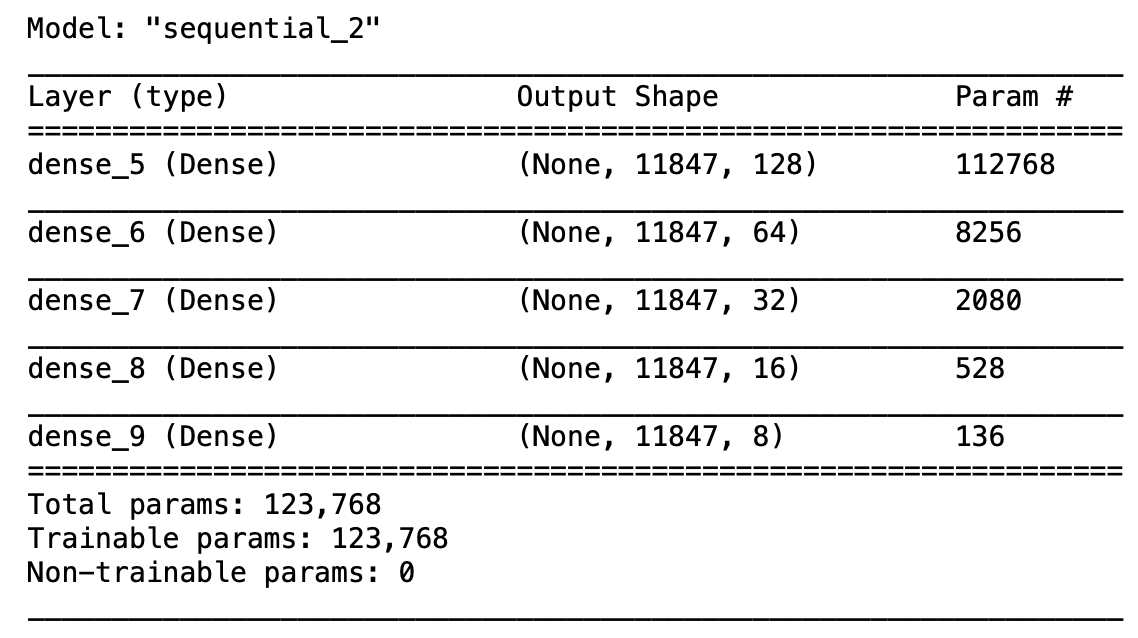
\includegraphics[width=\linewidth]{images/8 class model.PNG}
    \caption{8 speaker model}
    \label{fig:8 speaker model}
\end{figure}

\subsubsection{Random speaker recognition model}

Similar to the 8 speaker recognition model, we experimented with different layers and hyperparameters to get us the best result. We finally decided to use a similar network structure that we used for the 8-speaker recognition model, which is a 5-layer network. The first layer had the input size of 128 and the activation we chose was ReLU. The second layer has 64 as it’s input with ReLU activation. The third layer has 32 as it’s input with ReLU activation. The fourth layer has 16 as it’s input with ReLU activation. The final layer has a size of 50 with softmax activation. The optimizer used for the model was Adam with a learning rate of 3e-4. The loss was categorical cross entropy and the metric to analyze the model was accuracy. The total trainable parameters were 124,040. Figure \ref{fig:random speaker model} represents the model built to identify the 7 speakers and 1 “no-speaker” class.

\begin{figure}[h]
    \includegraphics[width=\linewidth]{{"images/random speaker model"}.PNG}
    \caption{Random speaker model}
    \label{fig:random speaker model}
\end{figure}

We chose a similar neural network model as the 8-speaker recognition model because we wanted to see which dataset helped us better recognize new speakers without prior training and didn't want to change too many variables in the experiment. We also chose a similar neural network structure because we wanted the output of the embedding vector to be the same size for the 8-speaker model and the random speaker model. 

%---------------EXP--------------
}
\subsection{Unsupervised speaker recognition} 

Once the model was trained using the training data, we saved the model locally to use it for the unsupervised speaker recognition phase. Similar to creating the training set for the supervised learning model, we extract the same features from each audio file and pass the test data to the model. Here, we do not want the classification result of the model i.e. we do not want the model to output one of the 8 speakers or the random speakers. Instead, we want to extract the embedding vector of the penultimate layer. So we popped the last layer from the model and now the output of the model is an embedding vector of size 16 for each audio file. The embedding vector looks like: 

[0, 0,  0,  0, 0, 57.781567,  0,   0,  44.595768,  0,  0,   13.87579,   0,  0,  0, 39.74966 ]

After obtaining the embedding vectors of each audio file, we use a clustering algorithm to figure out the number of clusters and which cluster each audio file belongs to. Each cluster represents a different speaker. For example, after running the clustering algorithm on the embedding vectors, we find out that there are 4 clusters. This means that there are 4 unique speakers in the group who are talking at different points of time. 

The clustering that we used is the hierarchical fclusterdata algorithm from the SciPy package. The SciPy documentation page  says that this algorithm “Clusters the original observations in the n-by-m data matrix X (n observations in m dimensions), using the euclidean distance metric to calculate distances between original observations, performs hierarchical clustering using the single linkage algorithm, and forms flat clusters using the inconsistency method with t as the cut-off threshold.”\cite{scipy}

\comment{
%---------------EXP--------------COMMENTED
We experimented with different hyperparameters to get the best results in terms of the correct number of clusters. For the hierarchical fclusterdata algorithm, we set criterion to distance, metric to euclidean, and method to centroid. We also had to choose a threshold for the clustering algorithm that worked best with different audio files and was accurate enough to predict the right number of clusters and which cluster each audio file belonged to.

There wasn’t an easy way to pick the right threshold. We ran the clustering algorithm with different thresholds and manually checked if the clustering algorithm grouped the audio files correctly. Figure \ref{fig: thresholds} shows an example of checking different thresholds.

\begin{figure}[h]
    \includegraphics[width=\linewidth]{{"images/thresholds"}.PNG}
    \caption{Testing different thresholds}
    \label{fig: thresholds}
\end{figure}

The threshold value we picked was 65, since it was the threshold which correctly identified the number of clusters for multiple different testing datasets. 

%---------------EXP--------------
}
\subsection{No speaker recognition model} 

A problem that we noticed while building the unsupervised speaker recognition model was that the clustering algorithm created a different cluster for instances when no one was speaking. Since we created a class called “no speaker”, the clustering algorithm clustered that as a speaker too.

In order to fix the problem, we had to create a no speaker recognition model, which is a binary neural network which outputs whether the audio file is a background noise without anyone speaking or if someone was speaking. In this instance there are only two classes.

\textbf{MODEL DESCRIPTION - need to fill}


While testing the unsupervised speaker recognition model, we first ran the 1 second audio file on the No speaker recognition model. If the model outputs “no speaker” then we just output that the audio file contains no speaker. If the model outputs “speaker” then we took that audio file and ran it through the 8-speaker recognition model or random speaker recognition model to get the embedding vector and then ran the clustering algorithm to find which speaker the audio file belonged to. This fixed the issue of the clustering algorithm considering background noises as a different cluster/speaker. This method also saves the extra cost of having to run an audio segment where no one is speaking through the entire large network.

\subsection{Live speaker recognition}

We created a python script to get a live stream of audio data from the computer, process every 1 second audio clip by extracting features on the audio and then the features get passed to the model to get the last layer embedding vector. The new embedding vector is added to a dictionary. This dictionary contains all the previous embedding vectors. That dictionary is then used to run the clustering algorithm to find which cluster that last added embedding vector belongs to. So every 1 second, the program will output the current speaker or “no speaker” if no one is talking. This is how an unsupervised speech recognition system works in real time.

%-----------------------------------------------------------

\section{Experiments}
This section describes all the experiments that we performed as part of this project. Section 4.1 describes the different experiments that we performed on the supervised speaker recognition model of the system, followed by section 4.2 which describes the experiments that we performed on the unsupervised speaker recognition model of the system.
\subsection{Supervised speaker recognition}
This part of the system consists of the actual neural network architecture. The input to this phase is the features extracted from the audio files, and the output is the embedding vectors of the penultimate layer of the network, which are used in the next phase for clustering.

We experimented with the following two different approaches for this phase:
\begin{itemize}
    \item Train a neural network using a dataset containing 8 celebrity speakers
    \item Train a neural network using a dataset containing random speakers
\end{itemize}
For both of these approaches, we experimented with various sizes of network layers, activation functions and other hyperparameters, and have described the options that gave the best results in the subsequent sections.
\subsubsection{8-speaker dataset}

The YouTube videos that we chose to include in this dataset were speeches/monologues from celebrities. We thought this would be the best way to build a labeled dataset of audios of different people. The dataset, shown in table \ref{tab:8-speaker-dataset} includes 7 celebrities (Obama, Hillary, Ivanka, Trump, Modi, Xi-Jinping, and Chadwick-Boseman) and one “no speaker” class which includes multiple background noises without anyone speaking. We included the “No Speaker” class so that the model can recognize when no one is speaking.  We wanted the dataset to be as diverse as possible, that is why we included speakers of both genders, different races, and also different languages. This dataset has a size of 4.1+ hours. 


\begin{table}[h]
    \begin{tabular}{l|l|l|l|l|}
    \cline{2-5}
                                                    & \textbf{Gender} & \textbf{Language} & \textbf{Race} & \textbf{Length} \\ \hline
    \multicolumn{1}{|l|}{\textbf{Obama}}            & Male            & English           & Black         & 19.5 mins       \\ \hline
    \multicolumn{1}{|l|}{\textbf{Hillary}}          & Female          & English           & White         & 57.5 mins       \\ \hline
    \multicolumn{1}{|l|}{\textbf{Ivanka}}           & Female          & English           & White         & 17.9 mins       \\ \hline
    \multicolumn{1}{|l|}{\textbf{Trump}}            & Male            & English           & White         & 41.6 mins       \\ \hline
    \multicolumn{1}{|l|}{\textbf{Modi}}             & Male            & Hindi             & Asian         & 32.4 mins       \\ \hline
    \multicolumn{1}{|l|}{\textbf{Xi-Jinping}}       & Male            & Chinese           & Asian         & 11.18 mins      \\ \hline
    \multicolumn{1}{|l|}{\textbf{Chadwick}}         & Male            & English           & Black         & 27.1 mins       \\ \hline
    \multicolumn{1}{|l|}{\textbf{No Speaker}}       & N/A             & N/A               & N/A           & 39.6 mins       \\ \hline
    \end{tabular}
    \caption{Details of the 8 speaker dataset}
    \label{tab:8-speaker-dataset}
\end{table}

\subsubsection{8-speaker model}

To build the 8-speaker recognition model, we experimented with different number of layers and hyperparameters to check which architecture achieved the best results. We finally chose the following 5-layer network:

\begin{itemize}[itemsep=-5pt]
    \item Layer 1 - Input size: 128, Activation: ReLU
    \item Layer 2 - Input size: 64, Activation: ReLU
    \item Layer 3 - Input size: 32, Activation: ReLU
    \item Layer 4 - Input size: 16, Activation: ReLU
    \item Layer 5 - Input size: 8, Activation: Softmax
\end{itemize}



\begin{figure}[h]
    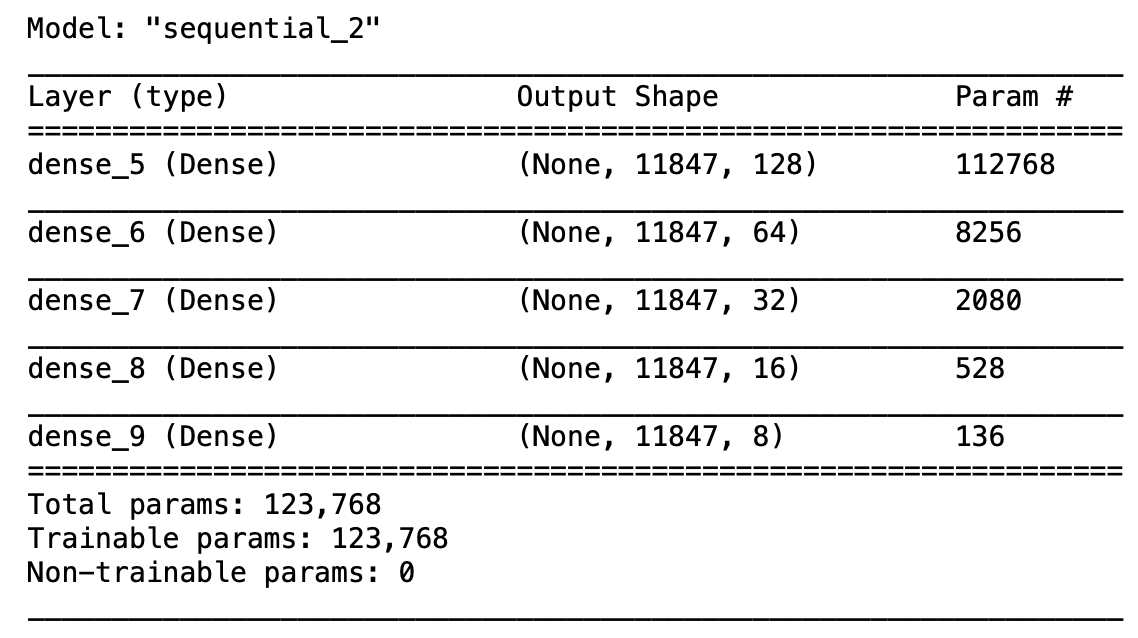
\includegraphics[width=\linewidth]{images/8 class model.PNG}
    \caption{8 speaker model}
    \label{fig:8 speaker model}
\end{figure}

The optimizer used for the model was Adam with a learning rate of 3e-4. The loss was categorical crossentropy and the metric used to evaluate the model was accuracy. The total number of trainable parameters were 123,768. Figure \ref{fig:8 speaker model} represents the model built to identify the 7 speakers and 1 “no-speaker” class.

This model achieved validation accuracy of around 99\% on the data, and a loss of around 0.07. Figure \ref{fig: 8 speaker model - accuracy} shows the graph for validation accuracy over time, and Figure \ref{fig: 8 speaker model - loss} shows the graph for the loss.

\begin{figure}[h]
    \includegraphics[width=\linewidth]{{"images/8 speaker - accuracy"}.PNG}
    \caption{8 speaker model - accuracy}
    \label{fig: 8 speaker model - accuracy}
\end{figure}

\begin{figure}[h]
    \includegraphics[width=\linewidth]{{"images/8 speaker - loss"}.PNG}
    \caption{8 speaker model - loss}
    \label{fig: 8 speaker model - loss}
\end{figure}


\subsubsection{Random speaker dataset}

We wanted to experiment on the quality and quantity of our dataset to see the impact on the speaker recognition model. The dataset that we created before only had 8 speakers but each speaker had multiple videos combining to more than 30 minutes each. In the dataset of random speakers, we got audio files of length 2-3 minutes of \textbf{50 speakers}. In this dataset we increased the amount of speakers but limited the number of audio files to 1 audio file (2-3 minutes) per speaker. 

The audios of the speakers were obtained from random YouTube videos and voice recordings. We only chose audios which had only one speaker speaking in the whole audio file and checked if there were no background music or sound. We limited the audio file to 2-3 minutes so we could have multiple speakers. Table \ref{tab:random-speaker-dataset} is a snippet of the YouTube videos used to create the random speaker dataset.

\begin{table}[h]
        \begin{tabular}{|l|l|l|}
        \hline
        \textbf{YouTube Title}                                       & \textbf{Length} \\ \hline
        How to evaluate expressions with two variables               & 2:04                         \\ \hline
        2020 Rock \& Roll Hall of Fame Speech                        & 2:31                         \\ \hline
        A look at U.S. President-elect Joe Biden                     & 3:32                         \\ \hline
        Open Office Math                                             & 2:46                         \\ \hline
        How to Get Stuff Done When You Have ADHD                     & 4:45                         \\ \hline
        How Online Math Tutoring via Skype Works                     & 2:38                         \\ \hline
        \end{tabular}
        \caption{A snippet of random speaker dataset}
        \label{tab:random-speaker-dataset}
\end{table}

\subsubsection{Random speaker model}

Similar to the 8-speaker recognition model, we experimented with different layers and hyperparameters. We decided to use a network architecture similar to the one we used for the 8-speaker recognition model, which is a 5-layer network. The only difference is that the last layer has a different size, which corresponds to the number of speakers in the respective dataset (50 in this nodel versus 8 in the previous model).
\begin{itemize}[itemsep=-5pt]
    \item Layer 1 - Input size: 128, Activation: ReLU
    \item Layer 2 - Input size: 64, Activation: ReLU
    \item Layer 3 - Input size: 32, Activation: ReLU
    \item Layer 4 - Input size: 16, Activation: ReLU
    \item Layer 5 - Input size: 50, Activation: Softmax
\end{itemize}

\begin{figure}[h]
    \includegraphics[width=\linewidth]{{"images/random speaker model"}.PNG}
    \caption{Random speaker model}
    \label{fig:random speaker model}
\end{figure}

The optimizer used for the model was Adam with a learning rate of 3e-4. The loss was categorical cross entropy and the metric to analyze the model was accuracy. The total trainable parameters were 124,040. Figure \ref{fig:random speaker model} represents the model built to identify the 50 random speakers.

This model achieved validation accuracy of around 92\% on the data, and a loss of around 0.5. Figure \ref{fig: Random speaker model - accuracy} shows the graph for validation accuracy over time, and Figure \ref{fig: Random speaker model - loss} shows the graph for the loss.

\begin{figure}[h]
    \includegraphics[width=\linewidth]{{"images/random speaker - accuracy"}.PNG}
    \caption{Random speaker model - accuracy}
    \label{fig: Random speaker model - accuracy}
\end{figure}

\begin{figure}[h]
    \includegraphics[width=\linewidth]{{"images/random speaker - loss"}.PNG}
    \caption{Random speaker model - loss}
    \label{fig: Random speaker model - loss}
\end{figure}

We chose a similar neural network model in this experiment as the 8-speaker recognition model because we wanted to see which dataset helped us better recognize new speakers without prior training and didn't want to change too many variables in the experiment. We also chose a similar neural network structure because we wanted the output of the embedding vector to be the same size for the 8-speaker model and the random speaker model, in order to effectively compare the results.

\subsection{Unsupervised speaker recognition}

We experimented with different hyperparameters to get the best results in terms of the correct number of clusters. For the hierarchical fclusterdata algorithm, we set criterion to distance, metric to euclidean, and method to centroid. We also had to choose a threshold for the clustering algorithm that worked best with different audio files and was accurate enough to predict the right number of clusters and which cluster each audio file belonged to.

There wasn’t an easy way to pick the right threshold. We ran the clustering algorithm with different thresholds and manually checked if the clustering algorithm grouped the audio files correctly. Figure \ref{fig: thresholds} shows an example of checking different thresholds.

\begin{figure}[h]
    \includegraphics[width=\linewidth]{{"images/thresholds"}.PNG}
    \caption{Testing different thresholds}
    \label{fig: thresholds}
\end{figure}

The threshold value we picked was 65, since it was the threshold which correctly identified the number of clusters for multiple different testing datasets.

\subsection{Results}

On comparing these two approaches, we found that the random speaker model performed better at the speaker recognition task despite the higher accuracy achieved by the 8-speaker model. We think this could be because the 8-speaker model is trained over recorded audio clips of celebrities, which are more likely to be recorded more carefully than the audio clips of random people. For example, speeches/monologues from Hillary Clinton would be recorded with better sound equipment, a relatively controlled environment (where they may not be overlapping speakers) and better post-processing to remove noise, whereas a random person's audio clip would have more background noise and overlapping speech. The latter is the more common situation in the real world, and hence the random speaker model performs better in a general situation, which is what we are looking for. It is also possible that the model is able to learn better features due to a wider variety in the speakers. 

Figure \ref{fig: output} shows the output of the system for an audio file of length 16 minutes which has 4 unique speakers. The output depicts which speaker is speaking at every 1 second interval. The final model achieves a 94\% accuracy over this audio file. As can be seen in the figure, there are still a small number of instances where the model is confused about who is speaking, as evidenced by the fluctuations. This could be because of overlapping speech, or similarities in the voice features of speakers. 

\begin{figure}[h]
    \includegraphics[width=\linewidth]{{"images/output"}.jpg}
    \caption{Final output}
    \label{fig: output}
\end{figure}

\section{Conclusion}

In this project, we have demonstrated that even relatively small and simple neural network approaches are quite capable of handling an unsupervised speaker identification task. We have also shown that novel combinations of supervised and unsupervised approaches can be leveraged to obtain effective models that have good performance over a given task.

Due to our computational resource constraints, we had to make use of relatively small datasets and simple networks. Future work in this domain could leverage larger datasets (like the VoxCeleb2 dataset \cite{base}) containing a larger number of speakers, or make use of more complex networks to develop more powerful models. These powerful models could be trained to be more effective even with more background noise, or to have a higher accuracy with more overlapping speech samples, or where multiple speakers are speaking at the same time. Other techniques could be combined to obtain models which are capable of providing accurate transcripts of conversations/events, such as an audience clapping or cheering.

\printbibliography
\end{document}
